\documentclass[a4paper,10pt,twoside]{article}
\usepackage[utf8]{inputenc}
\usepackage[french]{babel}
\usepackage[T1]{fontenc}
\usepackage{amsmath}
\usepackage{amsfonts}
\usepackage{amssymb}
\usepackage{graphicx}
\usepackage{multicol}
\usepackage{array}
\usepackage{float}
\usepackage{epstopdf}
\usepackage[justification=centering]{caption}
\usepackage{caption}
\usepackage{subfig}
\usepackage{gensymb}
\usepackage[bottom]{footmisc}
\usepackage{appendix}
\usepackage{pdfpages}
\usepackage{todonotes}
\usepackage{mathpazo}
\usepackage{titleps}
\usepackage{color}
\usepackage{hyperref}
\usepackage[skins]{tcolorbox}
\usepackage{sectsty} 
\usepackage[arrowmos]{circuitikz}
\usepackage{pgfplots}
\usepackage{blindtext}
\usepackage{adjustbox}
\usepackage[inner=2.5cm,outer=2.5cm,top=3cm,bottom=3cm]{geometry}

\graphicspath{{figures/}}
\setlength\parindent{0pt}
\renewcommand*\rmdefault{ppl}
\newcolumntype{C}[1]{>{\centering\let\newline\\\arraybackslash\hspace{0pt}}m{#1}}
\newcolumntype{R}[1]{>{\raggedright\arraybackslash}p{#1}}
\sectionfont{\large}
\subsectionfont{\normalsize}

% Page style definitions
\newpagestyle{main}{
	\sethead[Club ELEC : Hands-on 3][][]  % even
			{\chaptertitle}{}{Club ELEC : Hands-on 3}
	\headrule
    \setfoot[\thepage][][]
    		{}{}{\thepage}		
}

\newpagestyle{appendix}{
	\sethead[Club ELEC : Annexes][][]  % even
			{}{}{Club ELEC : Annexes}
	\headrule
    \setfoot[\thepage][][]
    		{}{}{\thepage}
    \footrule
}

%----------------------------------------------------------------------------------------
%	TITLE SECTION
%----------------------------------------------------------------------------------------
\title{	
	\vspace{2.5cm}
	\normalfont \normalsize 
	\huge Club ELEC\\ 
	\vspace{2.5cm}
	\huge Projet Audio\\
	\vspace{.25cm}
	\Large HO3 - Distorsion du signal audio
	\vspace{2.5cm}
	\centering
}

\begin{document}
\renewcommand{\figurename}{Figure}
\renewcommand{\thepage}{\roman{page}}
\setcounter{page}{1}

\pagenumbering{gobble}
\maketitle
\newpage
\pagenumbering{arabic}
\pagestyle{main}

\newpage
\null
\thispagestyle{empty}
\newpage
\clearpage

\setcounter{page}{1}

%%% Introduction
\section*{Introduction}
Pendant ce quadrimestre, le Club ELEC vous propose de développer une chaine de conditionnement pour un signal audio, provenant par exemple d'un ordinateur, smartphone, etc. Pour ce faire, le développement du circuit se déroulera en 3 phases, chacune correspondant à une séance de hands-on proposée par le club.

\begin{itemize}
	\item[-] HO1: Contrôle du volume sonore.
	\item[-] HO2: Filtrage du contenu fréquentiel.
	\item[-] HO3: Distortion du signal audio.
\end{itemize}

%%% Objectifs du HO2
\section*{Objectifs}
% Objectifs: prise en main du micro et du signal sonore, notion AC/DC, utilisation de l'oscilloscope, découplage AC

Les objectifs du premier hands-on sont:

\begin{itemize}
	\item[-] De se familiariser avec le matérial de base (breadboard, multimètre, oscilloscope) et les composants de base (résistances, capacités, amplificateurs opérationnels, composants intégrés) propres à l'électronique.
	\item[-] De comprendre le fonctionnement du micro qui assure la transduction du signal sonore en signal électrique.
	\item[-] De faire le lien entre le signal obtenu et son contenu fréquentiel afin de comprendre la notion de filtrage.
	\item[-] De comprendre la notion AC/DC et le découplage AC.
	\item[-] D'implémenter en pratique la première partie du circuit (micro, filtre et découplage).
\end{itemize}

\begin{figure}[!ht]
	\centering
	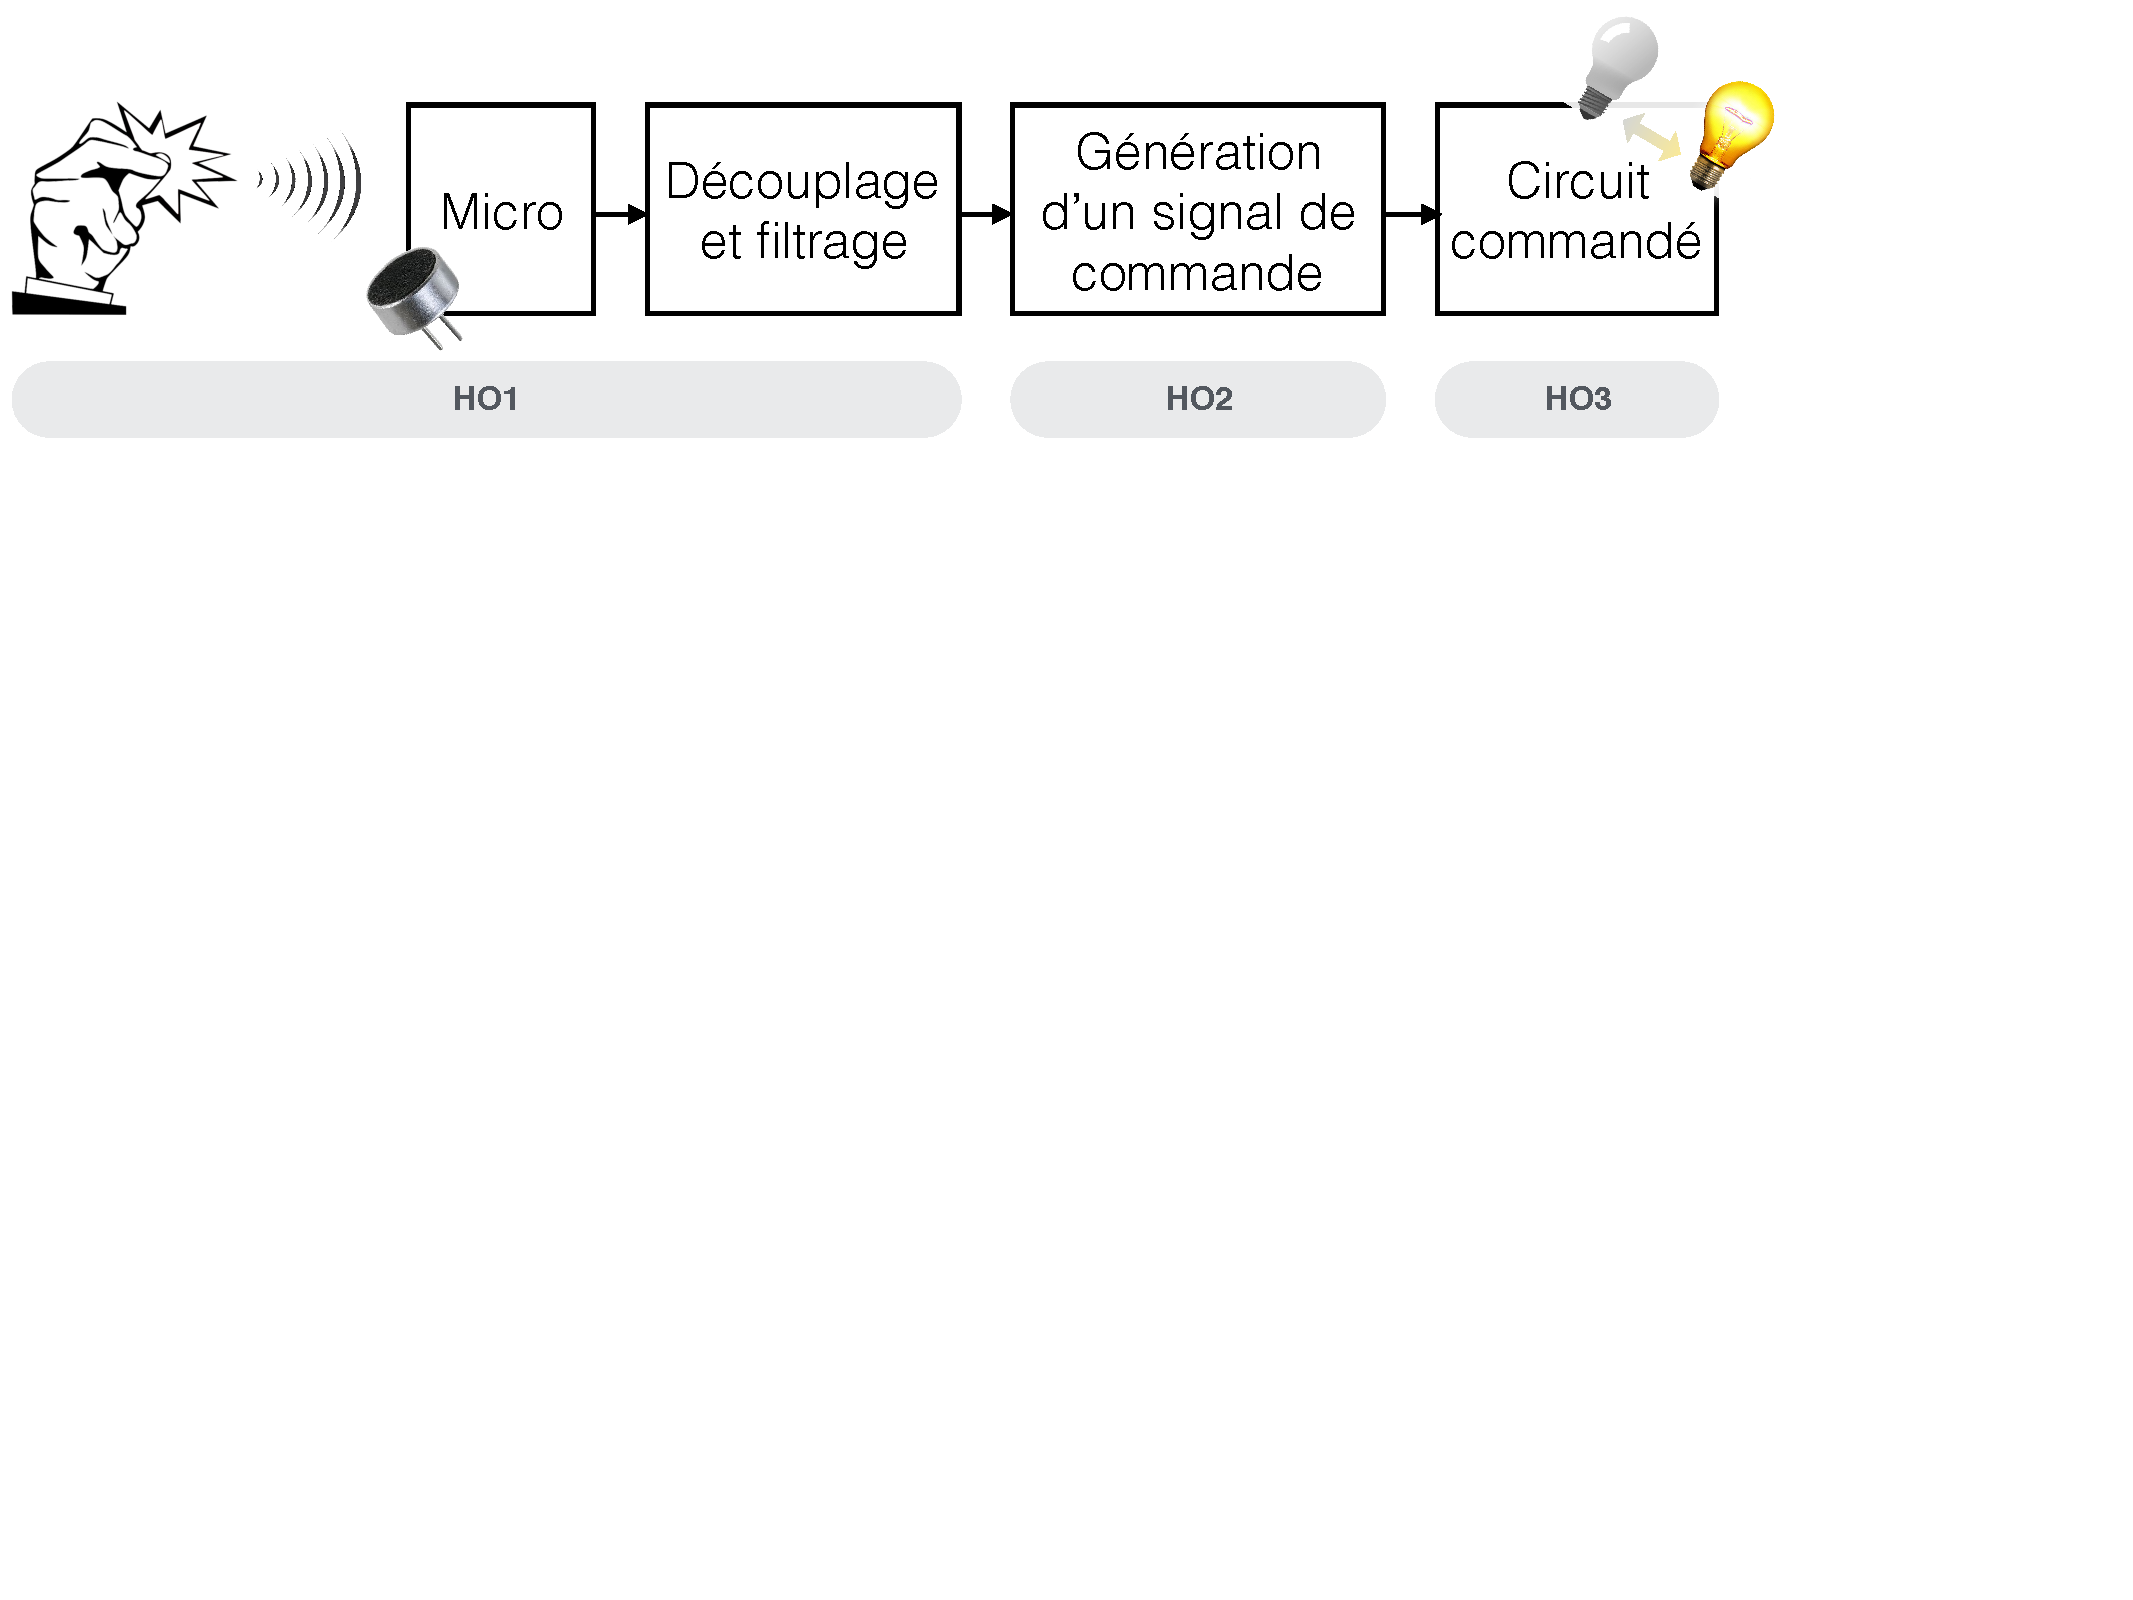
\includegraphics[width=.75\textwidth]{figures/SchemaBloc.pdf}
	\caption{Schéma-bloc du circuit.}
	\label{fig:block-diagram}
\end{figure}

Le schéma-bloc du circuit est présenté à la Figure \ref{fig:block-diagram}. Les ondes acoustiques générées par le claquement de doigt sont captées par le micro qui les transforme en un signal électrique (transduction). Ce signal est ensuite découplé et filtré à l'aide d'un filtre RC, comme présenté plus loin dans ce document. La génération d'un signal de commande propre ainsi que l'implémentation d'un circuit commandé seront abordées plus en détail dans les prochain hands-on.


\newpage

%%% Description du circuit
\section*{Description du circuit}
\begin{figure}[ht!]
	\centering
	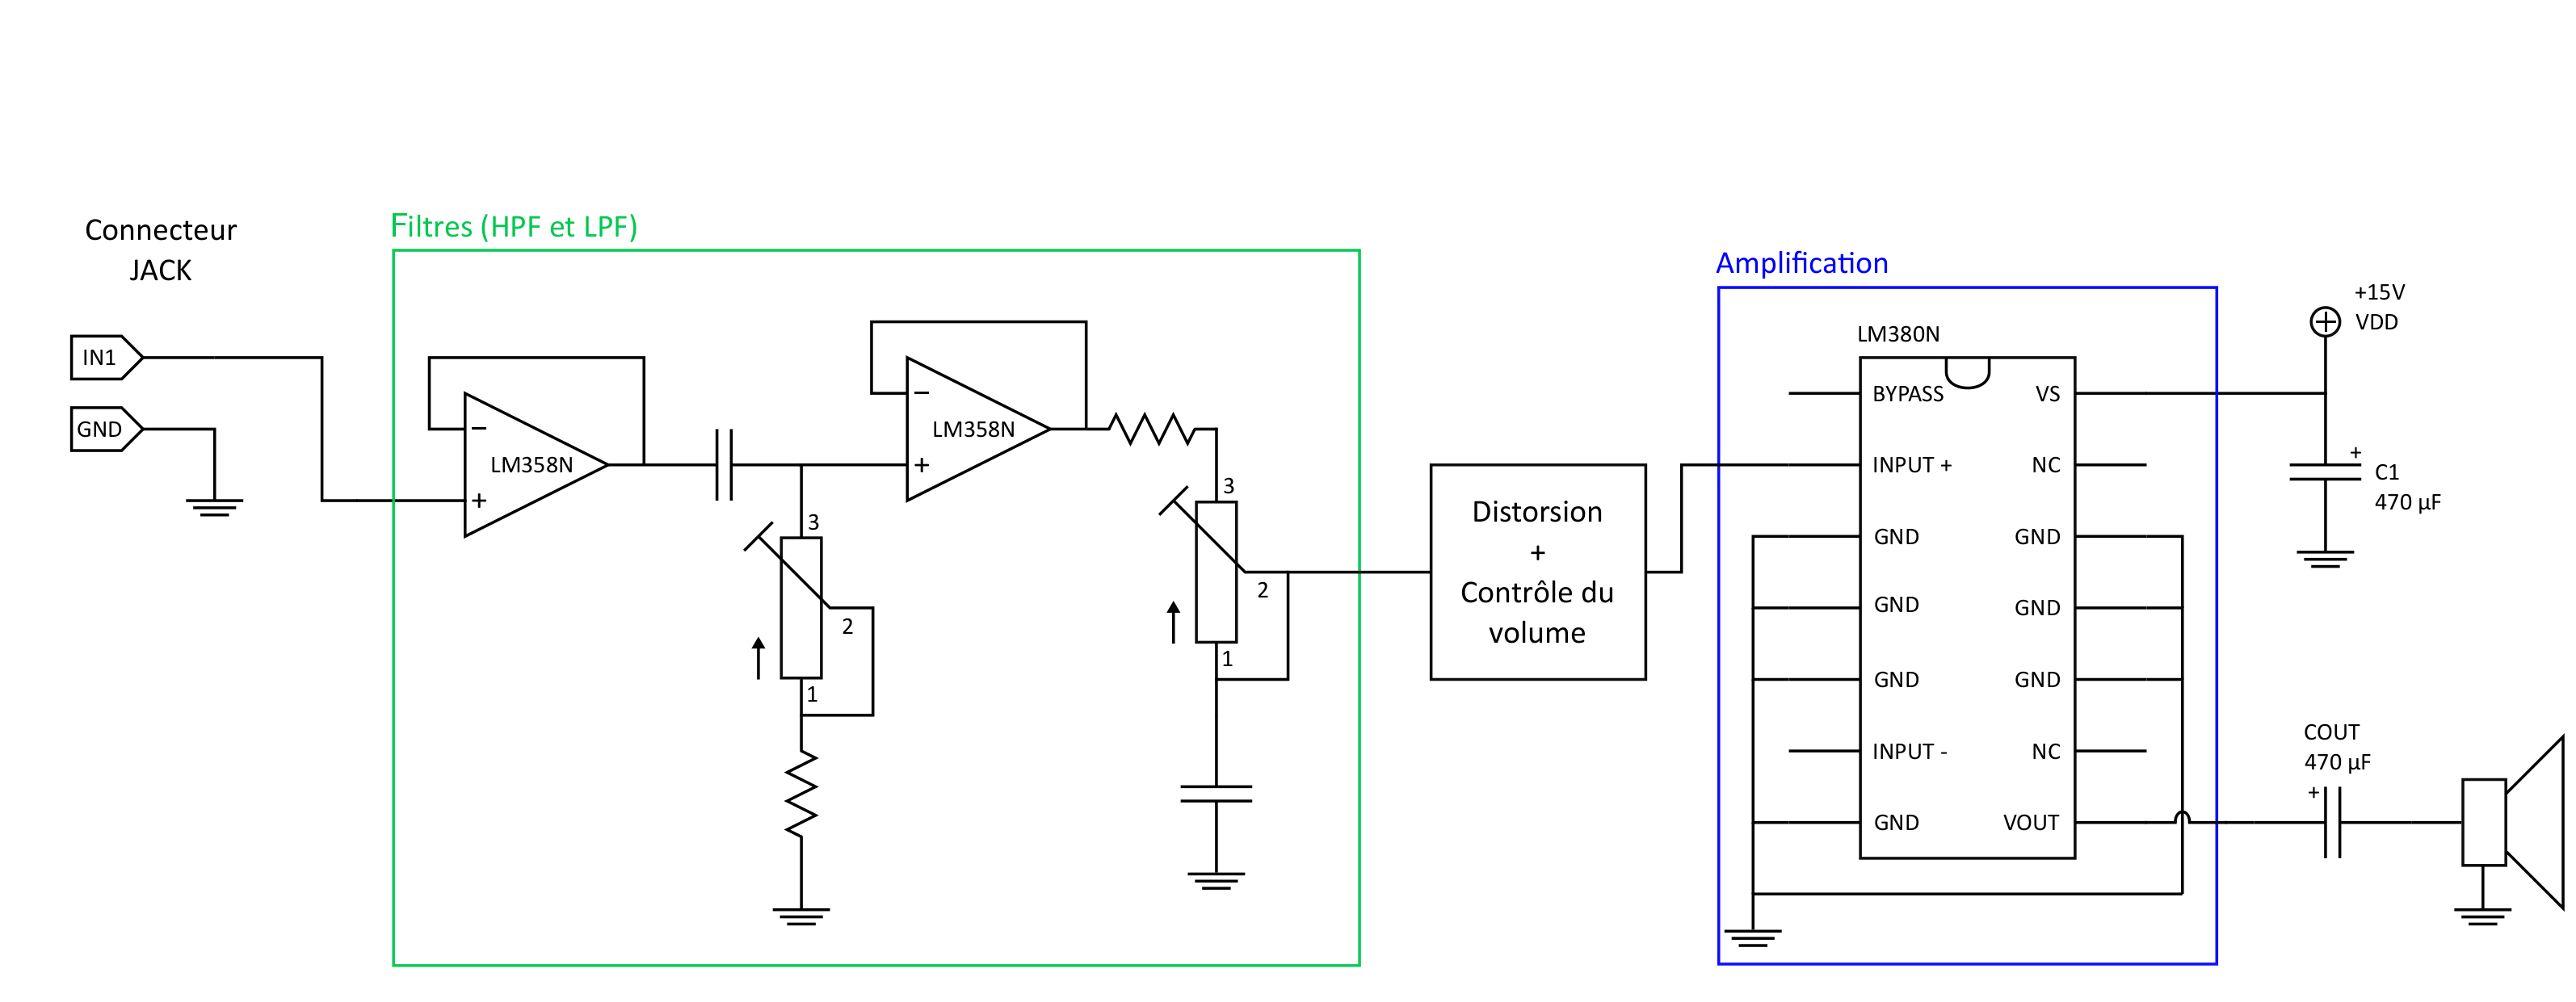
\includegraphics[width=\textwidth]{schematics}
	\caption{Schématique du circuit.}
	\label{fig2:schematics}
\end{figure}

Le schématique du circuit modifié est présenté à la Figure \ref{fig2:schematics}. En partant de la gauche, le signal d'entrée fourni par le câble jack à la borne IN1 passe d'abord dans le bloc de filtrage. Les filtres ont été implémentés sur base de topologies passe-haut et passe-bas passives, c'est-à-dire qu'elles n'utilisent pas d'amplificateur opérationnel. Pour éviter que l'impédance d'entrée (resp. sortie) des blocs suivants (resp. précédents) ait un impact sur le comportement des filtres, ceux-ci sont isolés du reste du circuit par des montages suiveurs, à savoir un amplificateur opérationnel avec une rétroaction unitaire sur la borne négative.Le signal est ensuite transmis au bloc de distorsion (de type overdrive/clipper), inspiré de la pédale appelée \textit{Dan Armstrong's Blue Clipper}. Le détail de ce circuit est présenté à la Figure \ref{fig3:clipper}. Ce bloc inclus également le contrôle du volume, implémenté par un diviseur résistif. Enfin, le signal est amplifié puis transmis au haut-parleur.

%\subsection*{Notions de distorsion}
%empty

\newpage

\subsection*{Circuit d'overdrive}
\begin{figure}[!ht]
	\centering
	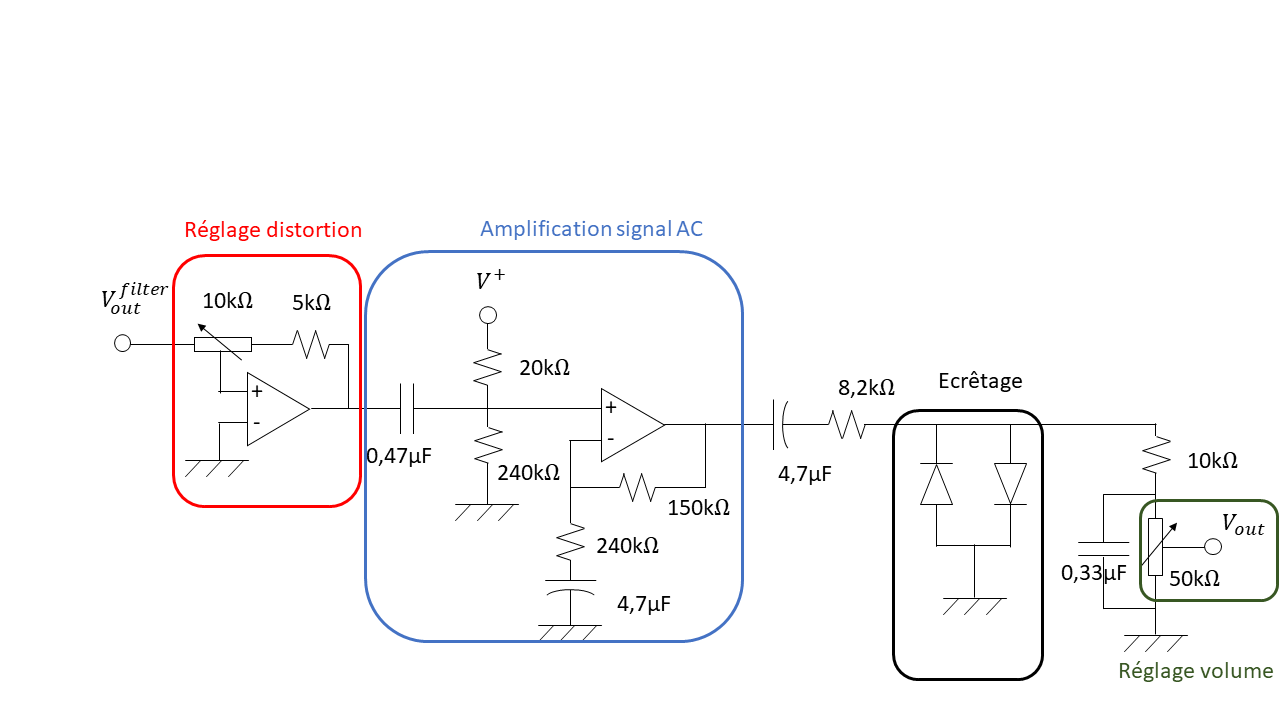
\includegraphics[width=.8\textwidth]{schematics-2}
	\caption{Schématique du bloc de distorsion et de contrôle du volume.}
	\label{fig3:clipper}
\end{figure}

Le circuit clipper permet d'introduire une distorsion dans le signal. Pour ce faire, les sinusoïdes sont remplacées par un signal carré. Le résultat sonore rajoute des grésillements au son original un peu comme sur une guitare électrique. Ce module est constitué des 4 éléments.  Les deux premiers sont utilisés afin d'amplifier le signal à distordre. Plus le signal entrant est amplifié, plus l'impact de la distorsion sera grand. En quelques mots, le bloc "réglage de distorsion" permet de régler via un potentiomètre l'amplification du signal et donc l'effet de la distorsion. Le bloc suivant permet d'amplifier uniquement la composante alternative de ce signal.

C'est le bloc "écrêtage" qui introduit la distorsion à l'aide de deux diodes. Ces diodes se comportent comme des courts circuits une fois une certaine tension à leurs bornes atteintes. Simplement, lorsque le signal d'entrée est supérieur à leur tension de seuil, la diode de droite devient passante avec la tension de seuil à ces bornes. Dans le cas d'un signal négatif inférieur à la tension de seuil, c'est la diode de gauche qui devient passante. Au final, les sinusoïdes à l'entrée de ce module sont transformées en signal carré. Le dernier bloc permet de régler le volume via un diviseur résistif.

Les Figures \ref{fig:ecret_pos} et \ref{fig:ecret_neg} donnent une idée de l'effet des diodes sur l'alternance positive et négative respectivement.

\begin{minipage}[c]{.49\textwidth}
	\centering
	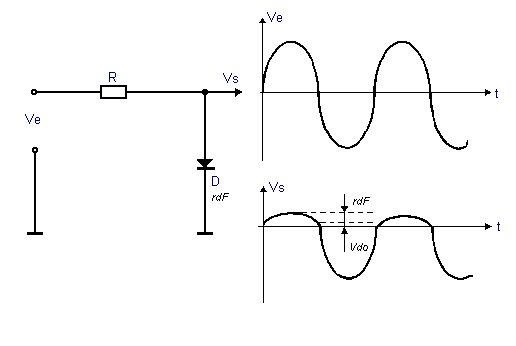
\includegraphics[width=\textwidth]{figures/ecret_pos.png}
	\captionof{figure}{Écrêtage de l'alternance positive.}
	\label{fig:ecret_pos}
\end{minipage}
\hfill
\begin{minipage}[c]{.49\textwidth}
	\centering
	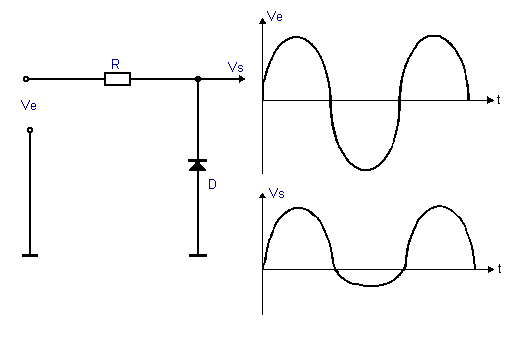
\includegraphics[width=\textwidth]{figures/ecret_neg.png}
	\captionof{figure}{Écrêtage de l'alternance négative.}
	\label{fig:ecret_neg}
\end{minipage}
\vspace{1cm}

\end{document}